% options:
% thesis=B bachelor's thesis
% thesis=M master's thesis
% czech thesis in Czech language
% slovak thesis in Slovak language
% english thesis in English language
% hidelinks remove colour boxes around hyperlinks

\documentclass[thesis=M,czech]{FITthesis}[2012/06/26]

\usepackage[utf8]{inputenc} % LaTeX source encoded as UTF-8

\usepackage{graphicx} %graphics files inclusion
% \usepackage{amsmath} %advanced maths
% \usepackage{amssymb} %additional math symbols

\usepackage{dirtree} %directory tree visualisation

% % list of acronyms
% \usepackage[acronym,nonumberlist,toc,numberedsection=autolabel]{glossaries}
% \iflanguage{czech}{\renewcommand*{\acronymname}{Seznam pou{\v z}it{\' y}ch zkratek}}{}
% \makeglossaries

\newcommand{\tg}{\mathop{\mathrm{tg}}} %cesky tangens
\newcommand{\cotg}{\mathop{\mathrm{cotg}}} %cesky cotangens


% XXX
%\setcounter{tocdepth}{4}
%\setcounter{secnumdepth}{4}


% % % % % % % % % % % % % % % % % % % % % % % % % % % % % % 
% ODTUD DAL VSE ZMENTE
% % % % % % % % % % % % % % % % % % % % % % % % % % % % % % 

\department{Katedra teoretické informatiky}
\title{Comma-shell, interaktivní debugger shellu}
\authorGN{Tomáš} %(křestní) jméno (jména) autora
\authorFN{Nesrovnal} %příjmení autora
\authorWithDegrees{Bc. Tomáš Nesrovnal} %jméno autora včetně současných akademických titulů
\supervisor{Ing. Jan Baier}
\acknowledgements{Doplňte, máte-li komu a za co děkovat. V~opačném případě úplně odstraňte tento příkaz.}
\abstractCS{V~několika větách shrňte obsah a přínos této práce v~češtině. Po přečtení abstraktu by se čtenář měl mít čtenář dost informací pro rozhodnutí, zda chce Vaši práci číst.}
\abstractEN{Sem doplňte ekvivalent abstraktu Vaší práce v~angličtině.}
\placeForDeclarationOfAuthenticity{V~Praze}
\declarationOfAuthenticityOption{4} %volba Prohlášení (číslo 1-6)
\keywordsCS{Nahraďte seznamem klíčových slov v češtině oddělených čárkou.}
\keywordsEN{Nahraďte seznamem klíčových slov v angličtině oddělených čárkou.}
\website{https://github.com/nesro/nesrotom-dip-2016} %volitelná URL práce, objeví se v tiráži - úplně odstraňte, nemáte-li URL práce

\begin{document}

% \newacronym{CVUT}{{\v C}VUT}{{\v C}esk{\' e} vysok{\' e} u{\v c}en{\' i} technick{\' e} v Praze}
% \newacronym{FIT}{FIT}{Fakulta informa{\v c}n{\' i}ch technologi{\' i}}

\begin{introduction}

Grafické uživatelské rozhraní (GUI) se jednoduše ovládá, ale ne vždy je k dispozici. To platí zejména při ovládání serverů.

Rozhraní příkazové řádky (CLI) je základní textové prostředí pro komunikaci s operačním systémem. Umožňuje spouštění programů, vkládat vstupní data a sledovat výstupní data v terminálu.

Jedním ze základních bodů UNIXové filosofie je mít jednoduché programy, které dělají pouze jednu věc, ale dělají ji dobře. To platí zejména pro základní příkazy ze sady GNU coreutils, tedy příkazy pro základní manipulaci se soubory, shellem a textem.

Tyto základní příkazy je možné řetězit a tím vytvářet užitečné jednořádkové skripty.

TODO: napsat o tom, ze pro začátečníka to může byt neintuitivní, musí si pamatovat spoustu příkazu. o návratových kódech, o historii prikazu a o logovani


\section{Motivace}

Příkazová řádka a základní práce s ní by měly být jedna z prvních věcí, které by se uživatel měl naučit, pokud chce umět používat svůj systém na vyšší úrovni. Stejně jako v programování platí, že počítač provádí dokonale a přesně to, co mu řekneme. Ale i při sebemenší chybě v našem příkazu selže celá sekvence akcí, které se měli provést. Není těžké udělat i nějakou fatální chybu, po které není snadné uvést vše do původního stavu.

Náš projekt, Comma-shell, si dává za úkol vytvořit z příkazové řádky místo, ve kterém je těžší nějaké chyby udělat, případně před chybou varovat, nebo vysvětlit, jak danou věc udělat lépe. Důležitý cíl je také umožnit nastavit toto prostředí tak, aby bylo snadno použitelné, nebylo potřeba externích terminálů, nebo grafických aplikací a aby bylo možné snadno omezit repetitivní výstupy programu. Comma-shell se dělí na tři části, každá pomáhá řešit jiný problém.

Comma-shell hooks, nebo-li části kódu, které lze vykonat před, nebo po vykonání spuštěného příkazu a dokonce zabránit jeho spuštění umožňují ochránit uživatele před vykonáním příkazu, který je v například nějakém smyslu nesprávný, špatný, nebo je v nepořádku. Pokud tedy napíše příkaz, který obsahuje nějaký překlep, nebo chybu, která by způsobila neočekávané chování, může být uživatel varován, než bude takový příkaz proveden. Nejde jen o ochranu uživatele před špatnými příkazy. Díky informacím o spouštěném příkazu a následně o jeho výsledku lze psát různé skripty, které by jinak bylo složité vytvořit.

Comma-shell debugger, tedy ladící program pro příkazy spouštěné z interaktivní příkazové řádky. Pokud uživatel píše složitější program, obsahující například smyčku, nebo roury a příkaz nefunguje tak, jak uživatel očekává, tak nejjednodušší je rozdělit si příkaz na podpříkazy a ujistit se, že každý příkaz dělá to, co od něj uživatel očekává. Comma-shell debugger by měl tento postup automatizovat.

Poslední částí jsou takzvané bezpečné příkazy. Pokud uživatel vykoná příkaz, jehož efekt byl jiný než očekával, chce spustit opačný příkaz, aby napravil svůj omyl, nebo má často mnohem větší problém, pokud šlo například o nesprávné použití programu pro mazání souborů. Cílem bezpečných příkazů je tedy zaprvé umožnit vrátit provedené změny, ale i informovat uživatele o tom, co se stane. Pokud uživatel používá ke specifikování souborů, které mají být cílem nějakého příkazu, je častý omyl vybrat nějaké soubory nechtěně. Nebo například provést příkaz ze špatného adresáře.


% https://www.gnu.org/software/coreutils/coreutils.html
% http://www.tldp.org/LDP/GNU-Linux-Tools-Summary/GNU-Linux-Tools-Summary.pdf

% https://en.wikipedia.org/wiki/Unix_philosophy
% ^- tady je spousta dalsich uzitecnych odkazu, o cem by se mohlo psat

% https://en.wikipedia.org/wiki/Command-line_interface
% https://en.wikipedia.org/wiki/Shell_(computing)
% https://www.abclinuxu.cz/ucebnice/zaklady/prikazova-radka

\end{introduction}

\chapter{Definice a pojmy}

Příkazová řádka, anglicky Command Line Interface, je uživatelské rozhraní ovládané příkazy. Příkazy spuštěné z příkazové řádky vypisují výstup také na příkazovou řádku a další interakce se spuštěným programem probíhá zase zadáváním příkazů. Na rozdíl od textového nebo grafického rozhraní uživatel nemůže nijak zasahovat do již vypsané či vykreslené části.

TODO: obrazek prikazove radky, tui a gui
% https://cs.wikipedia.org/wiki/Textov%C3%A9_u%C5%BEivatelsk%C3%A9_rozhran%C3%AD

Shellem se obecně myslí uživatelské prostředí pro využívání funkcí jádra operačního systému. V této práci budeme slovem shell označovat právě interpret příkazů v příkazové řádce. Tedy program, ovládaný příkazy, který umí spouštět ostatní programy a zajišťovat jejich vstup a zobrazovat jejich výstup.

Prompt je krátký řetězec znaků, který se objeví na začátku řádky, do které se bude vepisovat příkaz v příkazové řádce. Je používán k zobrazování důležitých informací, jako například, ve kterém adresáři se uživatel nachází či jaké je jméno počítače, na kterém se nachází.
% http://www.linfo.org/prompt.html


GNU je projekt zabývající se tvorbou a propagací svobodného software. Cílem je vytvořit kompletní svobodný operační systém unixového typu. Protože jádro operačního systému od GNU s názvem Hurd nebylo tak úspěšné, začalo se používat jádro Linux. Kombinace operačního systému GNU a jádra Linux se označuje jako GNU/Linux. GNU vytvořilo i svůj shell, Bash. Sada základních příkazů, jejichž existence je předpokládána v nějaké formě na každém operačním systému, se jmenuje GNU coreutils. Patří do ní příkazy jako ls, cp, rm, atd. Je důležité si uvědomit, že příkazy jako cd, echo jsou vestavěné příkazy shellu Bash.

% https://www.gnu.org/software/bash/
% https://www.gnu.org/software/coreutils/coreutils.html

Terminál byl z historického hlediska elektronické zařízení k základní komunikaci s počítačem. Dnes se v operačních systémech spouští terminálové emulátory, ve kterých lze spustit různé programy. Nejčastěji je to právě shell.


Provádění příkazů můžeme rozdělit na dvě kategorie. Jednou z nich je interaktivní režim, kdy interpret spouští příkazy tak, jak je uživatel píše do příkazové řádky. V tomto režimu může uživatel také používat klávesové zkratky, aliasy, automatické doplňování a další funkce v interaktivním režimu. Druhou kategorií je dávkový režim, kdy uživatel nejprve příkazy napíše do souboru. Takovému souboru obsahujícímu příkazy se říká skript. Takový soubor může být zavolán interpretem shellu, který postupně vykoná všechny příkazy. Tento postup se hodí pro složitější a opakující se příkazy.

\chapter{Historie shellu a dnešní využití}

Napsat o tom, ze bash je dneska nejcastejsi, protoze linux je vlastne GNU/Linux a bash je GNU bash. Zsh je lepsi snad uplne ve vsem. Sh, resp Dash je rychlejsi.

\section{UNIX}

Unix je rodina operačních systémů, které zvládnou spustit více úkonů najednou a do kterých se v jeden okamžik může připojit více uživatelů. Historie těchto sytému sahá až na konec sedmdesátých let, kdy v Bell laboratořích firmy AT\&T byl v jazyce C vytvořen systém UNIX, jehož název byl zaregistrován jako ochranná známka. Časovou osu ukazuje obrázek \ref{fig:unixhistory}. Specifikace "Single UNIX Specification" je souhrn standardu, které operační systém musí splňovat a dodržovat, aby se mohl označovat za UNIX.

Filosofie Unixu je sada doporučení a pravidel, která vznikla postupem času dle zkušeností tvůrců Unixu. Filosofie Unixu zdůrazňuje tvoření jednoduchého, přehledného a hlavně snadno rozšiřitelného a znovupoužitelného softwaru. Váží si programátorův čas více, než čas práce počítače. Nejznámější pravidlo je tvořit programy, které dělají jen jednu věc a dělají jí správně, rychle a bez chyb. Takové programy lze použít jako filtry a skládat je za sebe. To se často používá v příkazové řádce, kdy se pomocí rour spojují výstupy programů se vstupy jiných programů. Zdánlivě složitý úkol tak lze udělat rychle a efektivně bez nutnosti programování v nějakém jazyce.


\begin{figure}
	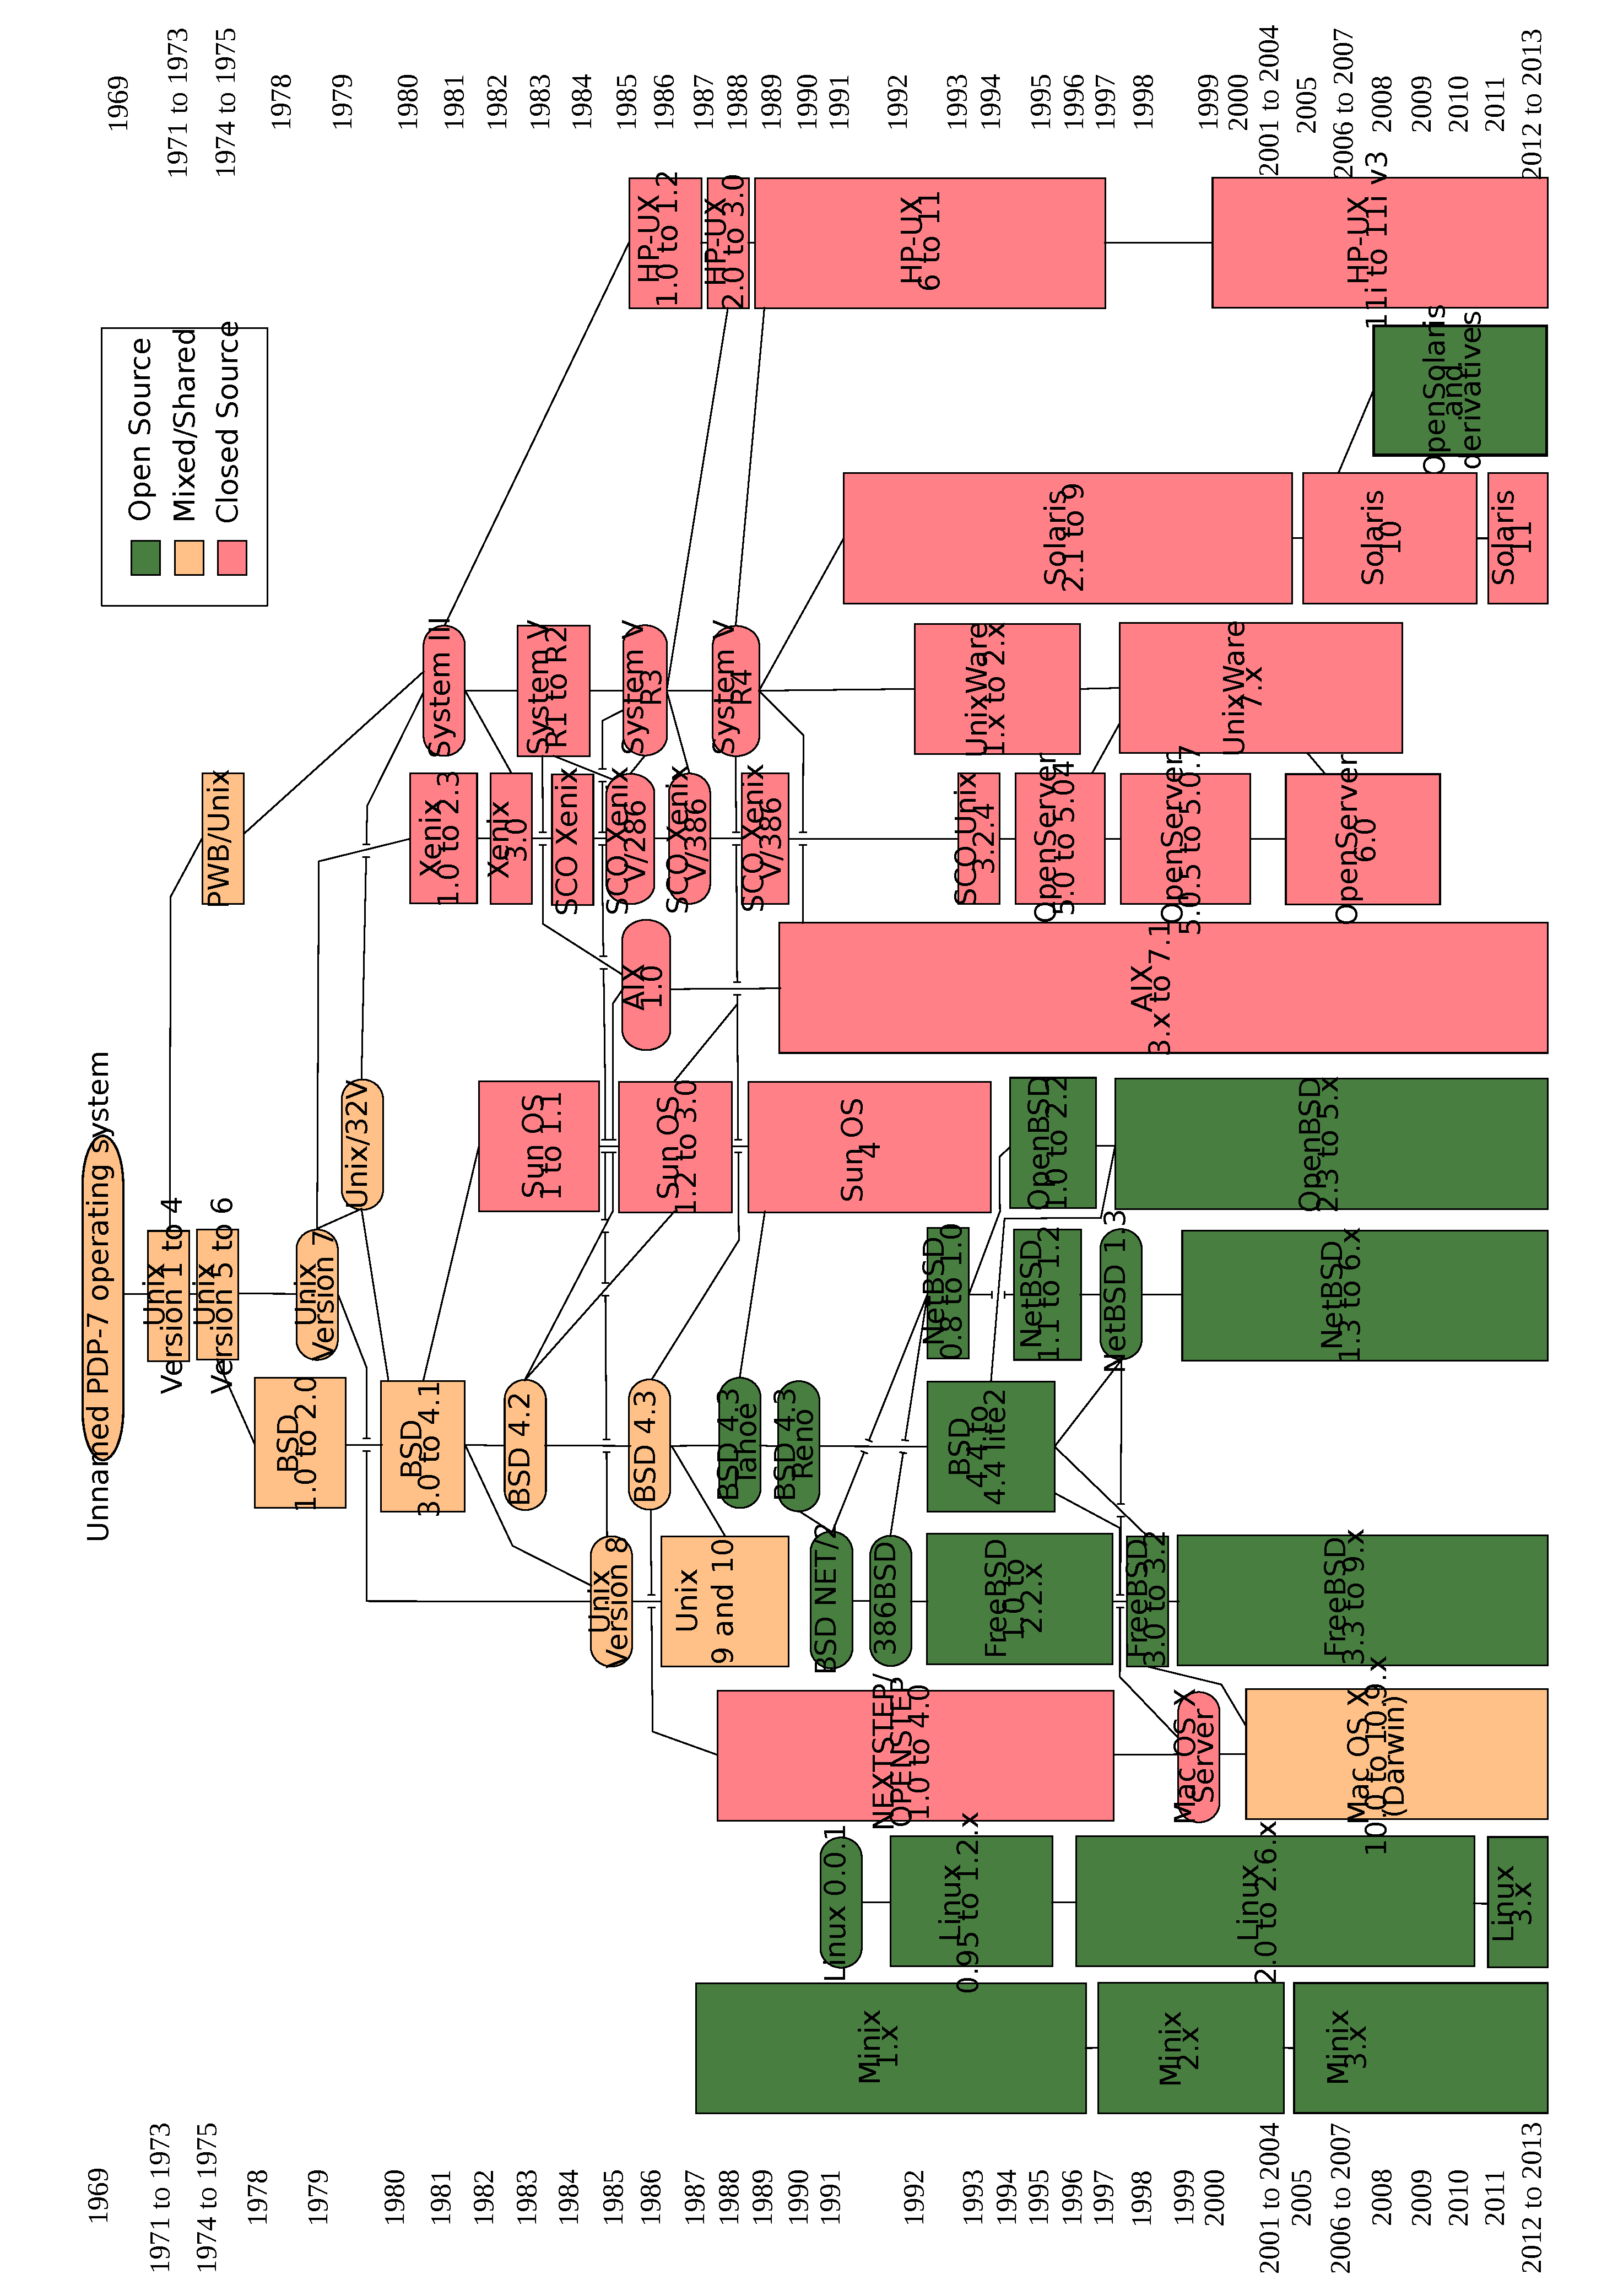
\includegraphics[width=1.0\textwidth]{./images/Unix_history-simple_rot_big}
	\caption{Historie unixu}
	\label{fig:unixhistory}
\end{figure}

% https://en.wikipedia.org/wiki/File:Unix_history-simple.svg
% XXX: mozna https://simple.wikipedia.org/wiki/File:Unix_timeline.en.svg ?

% ZDROJ: https://edux.fit.cvut.cz/courses/BI-PS1/_media/lectures/01/bi-ps1-p01-introduction-01.pdf

\section{Linux}
Linux je otevřený a svobodný Unix-like operační sytém. Linuxem se obecně myslí GNU operační systém s jádrem Linux. Unix-like znamená, že přestože je takový operační systém velice podobný systému Unix, nemá certifikaci "Single UNIX Specification". Linuxová distribuce je GNU/Linuxový systém, který většinou obsahuje balíčkovací systém, kterým je snadné doinstalovat ostatní programy. Linuxové distribuce jsou i předpřipravené, s grafickým prostředím. Například v této práci ukazujeme návod na vytvoření takového připraveného systému, GNU/Linuxové distribuci Debian s předpřipraveným grafickým prostředím LXDE a aplikacemi z rodiny LXDE.


% https://www.amazon.com/Just-Fun-Story-Accidental-Revolutionary/dp/0066620732

% unix timeline for students
% http://unix.harley.com/instructors/timeline.html
% http://www.harley.com/books/sg3.html

% Recommended UNIX Books
% http://www.it.northwestern.edu/research/user-services/sscc/booklist.html

% https://www.goodreads.com/book/show/104745.The_Art_of_UNIX_Programming

\section{Shell}

\begin{figure}[htb]\centering
	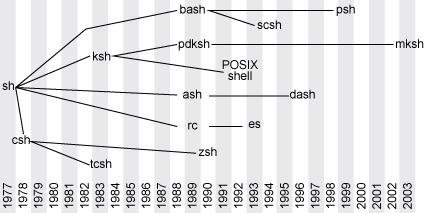
\includegraphics[width=\textwidth]{./images/tmp_shell_history}
	\caption{Historie Shellu}
	\label{fig:shell_history}
\end{figure}

V latexovych komentarich jsou nejake odkazy o historii.

% uvod, prehled csh, ksh, bash.
% https://www.ibm.com/developerworks/library/l-linux-shells/

% clanek od bourna z 1983, uvod do shellu, drtiva vetsina plati i dneska
%https://ia800300.us.archive.org/1/items/byte-magazine-1983-10/1983_10_BYTE_08-10_UNIX.pdf

% puvodni shell z unix v6
%https://github.com/JNeitzel/v6shell




\section{Bash - Bourne Again Shell}

\url{https://cs.wikipedia.org/wiki/Debian_Almquist_shell}
\url{https://wiki.archlinux.org/index.php/Dash}

\section{Sh - Bourne Shell}

todo

\section{Dash - Debian Almquist Shell}

todo

\section{Zsh - Z Shell}

todo

\url{http://zsh.sourceforge.net/FAQ/}

\section{Práce v příkazové řádce}
todo: tady bych chtel shrnout obecne to, ze se pisou prikazy jako text a uzivatel vse vidi jako text. co z toho plyne za nasledky a jak je snadne udelat chybu

\section{Nastavení shellu}

GNU/Linuxové distribuce, které nabízejí předpřipravené prostředí, mají pro výchozí shell bash připravené takzvané rc soubory, které nějakým způsobem upravují běžící interaktivní shell. Jednou z nejviditelnějších změn je nastavení proměnné PS1, o které bude řec v pozdější kapitole, která určuje styl promptu. Ve výchozím nastavení bashe, tedy po spuštění bashe bez načtení rc souborů (bash --norc), se v PS1 zobrazuje pouze název shellu, jeho verze a zdali je uživatel root. Po načtení výchozích rc souborů se v PS1 ukazují informace jako je například jméno uživatele, jméno počítače a co je velmi důležité, jméno aktualního adresáře.

Tyto informace jdou snadno získat použitím některých základních příkazů, například whoami, hostname, pwd. Protože tyto informace jsou důležité a potřebujeme je vedět pořád, chceme je mít pořád na očích.

\section{Terminál}
todo: asi by se hodilo napsat i neco o tech programech, ve kterych shell bezi

%-----------------------------------------------------------------------------


Napsat o tom, ze cilem prace je usnadnit praci v prikazove radce a sepsat zakladni funkcionalitu debuggeru.





\section{Existující řešení}

Mezi seznamem různých zajímavých řešeních awesome ( github.com/sindresorhus/awesome ) existuje i podsekce awesome-shell ( github.com/alebcay/awesome-shell ), ve které lze nalézt spoustu užitečných nástrojů pro práci s příkazovou řádkou, nebo psaním skripů v bashi.

Spousta těchto nástrojů je nad rámec této práce. 


\section{Bash frameworky pro psaní skriptů}

Existuje mnoho projektů, jejiž cílem je vytvořit framework v bashi, který má nějakým způsobem zjednodušit vytváření, především větších, skriptů v bashi. Spousta dnešních vývojářů je zvyklá na objektově orientovaný přístup k programovaní a je tedy pro těžké vytvořit větší program, který by zůstal přehledný.

\subsection{Bash OO framework}
Bash OO framework ( \url{github.com/niieani/bash-oo-framework} ) je framework napasny v bashi, ktery umoznuje vytvaret tridy, vyjimky a testy. Jeho cilem je vytvorit prostredi pro psani skriptu, kde se bude snadneji psat citelny kod, bez casti, ktere se opakuji.

%
%
%
%
%

\section{Bash frameworky pro správu doplňků}

Existuje spousta věcí, které uživatel příkazové řádky potřebuje občas řešit. Řešení pro daný problém je víc. Buď si uživatel vyřeší problém sám, nebo bude hledat řešení na internetu. Shellovské frameworky, které umějí i spravovat doplňky, mohou mít řešení pro daný problém. Instalace a použítí pak bude velmi jednoduché, intuitivnií a bude zde nějaká záruka o fuknčnosti a kvalitě.

Přestože je tato práce převážně o shellu bash, zsh je v tomto mnohem rozšířenější.

\subsection{Oh My Zsh}

Oh My Zsh ( \url{ohmyz.sh} ) je framework pro Zsh.

\subsection{Bash-it}

Bash-it ( \url{http://github.com/Bash-it/bash-it} )

( itsfoss.com/bash-it-terminal-tool/ ) 

%
%
%

\section{Bash frameworky pro úpravu promptu}

\subsection{Liquid Prompt}

Projekt liquidpromp \url{github.com/nojhan/liquidprompt} je adaptivní prompt v interaktivním bashi.

\subsection{Sexy Bash Prompt}

Projekt sexy-bash-prompt \url{https://github.com/twolfson/sexy-bash-prompt} je další používaný prompt v interaktivním bashi.

%------------------------------------------------------------------------------


\chapter{Analýza a návrh}

\section{Cíl práce}
todo




\section{Fungování shellu}

\subsection{Životní cyklus příkazu}

todo: popsat, co vsechno se stane, od napsani prikazu az po jeho vykonani

\subsection{Gramatika shellu}
Soubor s gramatikiou bashe, parse.y, ma pres 6000 radek. Chtel bych zde napsat zjednodusenou gramatiku, ktera by se dala snadno pochopit (ono to zas tak slozite neni).

Popsat jakym zpusobem parsuje gramatiku BASH (yacc) a jakym to delaji parsery bashlex a bashast.



\subsubsection{Projekty parsující shell}
https://github.com/bemeurer/beautysh/blob/master/beautysh/beautysh.py

\subsubsection{Bashlex}
https://github.com/idank/bashlex/blob/master/bashlex/parser.py

\subsubsection{Bashast}
https://github.com/neloe/libbash/blob/master/bashast/bashast.g


% https://github.com/idank/bashlex/blob/master/bashlex/parser.py
% https://github.com/neloe/libbash/blob/master/bashast/bashast.g

% https://stackoverflow.com/questions/5491775/how-to-write-a-shell-lexer-by-hand

\subsection{Spouštění příkazů}
Popsat základní principy jak funguje shell. Popsat procesy v unixu, fork, exec, co vsechno se musi stat, aby shell mohl spustit prikaz.

\subsection{Struktura BASHe}
todo: Zdrojovy kod je rozdelen do souboru, mozna by bylo dobre popsat popsat co ktery soubor dela, aby si ctenar udelal alespon trosku obrazek.

% bash git repo
% git clone git://git.savannah.gnu.org/bash.git

% buffering in standard streams
% http://www.pixelbeat.org/programming/stdio_buffering/

\section{Debugovaní shellu} %-------------------------------------------------

% ZADANI
tohle je jeden bod zadani: "Proveďte rešerši existujících nástrojů pro statickou analýzu, krokování a hledání chyb v BASH skriptech."

\subsection{Debugovaní Bashe}
todo: navod na debugovani bashe primo pomoci gdb. (tohle nakonec pro moji praci nebylo potreba) 

\subsection{Interní nástroje}

todo: popsat to, jake nastroje ma v sobe bash zabudovane v zakladu

\subsubsection{Debugovací mód BASHe (jak funguje shopt s extdebug)}
shopt s extdebug

\subsubsection{set x, u, v, e}
priklady do skriptu

\subsubsection{PS0, PS4}
PS0 bude v novém bashi, my ji proto nebudeme používat, PS4 se vypisuje při debugovaní.
todo: ps0 se nakonec nepovedlo

\subsection{Externí nástroje}

\subsection{BASH Debugger}
todo: popsat jak funguje, co vsechno umi, nejake priklady
\url{http://bashdb.sourceforge.net/}


\subsection{BashEclipse}
BashEclipse je plugin do Eclipse, ktery umi krokovat v gui eclipse.

\url{http://unix.stackexchange.com/questions/131491/is-there-a-gui-debugger-for-shell-scripts}
\url{https://sourceforge.net/projects/shelled/}
\url{https://sourceforge.net/projects/basheclipse/}

%
%
%
%
%
\section{Možnosti debugování v interaktivním shellu}

Nebyl nalezen žádný nástroj pro debugování interaktivního shellu. todo

\subsection{Definice debugování interaktivního shellu}
todo: nema cenu debugovat jednoduche prikazy, ale slozite ano. chceme umet rozkrokovat pipy a subshelly (tedy to co nam to dela ted)



\subsection{GNU Readline}
GNU Readline umožnuje přemapovat enter tak, abysme mohli spustit prikaz v nami definovane funkci. Problémem je, že takto upravený příkaz se uloží do historie. Dalším problémem jsou víceřádkové příkazy, tedy takové, pro jejichž napsání musíme několikrát zmáčknout enter.
TODO: ukázka.

\subsection{Napsání nového REPLu}
Zprovoznění základní funkcionality by bylo snadné, vzhledem ke komplexnosti BASHe však téměř nemožné mít stejné chování jako v BASHi.

\subsection{DEBUG trap}
Současné řešení. Při zapnutém extdebug je možné příkazy nepustit a jen evalovat poslední příkaz z historie. TODO: je potřeba popsat základní chování historie (např mezera na začátku příkazu, atd.)




% https://bmizerany.github.io/roundup/


\section{Statická analýza skriptů}

bash ma validaci syntaxe: bash -n, ale to nezjisti skoro zadne chyby.

\subsection{Check Bashisms}
\url{http://checkbashisms.sourceforge.net/}
Některé skripty cheme kvůli rychlosti spouštět v Bourne-Shellu. Protože ten je pouze podmnožina bashe, tento nástroj najde výskyty syntaxe, která je podporovaná pouze v bashi a v Bourne-Shellu nemusí fungovat správně.

\subsection{Explain Shell}
Tato analýza nehledá chyby, ale vyparsuje vložený kód a vyhledá příslušnou dokumentaci v manuálových stránkách. Využívá knihovny bashlex, kterou využijeme v našem debuggeru.
\url{http://www.explainshell.com/}


\subsection{ShellCheck}
todo: tady bych se mohl rozepsat vic. o tom, ze to je napsane v haskellu, o tom ze existuje databaze veci, ktere se ve skriptech hledaji a ze ke kazdym je wiki..

%%%%%%%%%%%%%%%%%%%%%%%%%%%%%%%%%%%%%%%%%%%%%%%%%%%%%%%%%%%%%%%%%%%%%%%%%%%%%%%
\chapter{Realizace}

% ZADANI
v zadani je:
Navrhněte a implementujte nástroj, který umožní psát uživatelské skripty pro analýzu příkazů a ovlivňování jejich spouštění a vykonávání. = to jsou hooky

Nástroj musí umožňovat krokovat složitější skripty po jednotlivých příkazech. = to je debugger

Pro analýzu spouštěných skriptů využijte vhodný nástroj z rešeršní části. = to je shellcheck




%
%
%
%
%
\section{Nespouštění příkazů}
Pro zabránění spouštění používáme DEBUG trap.
todo: popsat problemy a reseni


%
%
%
%
%
\section{Implementace debuggeru}
todo: napsat o tom, ze cast je napsana v pythonu a ze se cela vec spousti v pre-hooku, takze to je presne ten cas, kdy se muze prikaz debuggovat a originalni prikaz se nespusti.

popsat parsovani v bashlex a jak se cela vec predava do bashe

%
%
%
%
%
\section{Hooks}
Aby byl kód přehledný, kromě bezpečných příkazů je funkcionalita je rozdělena do hooků, nebo-li modulů, které obsahují kód, který je spuštěn před, nebo i po vykonání příkazu. Kód vykonaný před příkazem může rozhodnout, zda-li má dojít k zabránění vykonání příkazu.


\subsection{Implementace hooků}
todo: napsat o tom, že se hooky pousti automaticky pred i po a ze je snadne vytvorit vlastni hook

\subsection{Hooky před vykonáním příkazu}
todo: napsat co všechno můžu dělat

\subsection{Hooky po vykonáním příkazu}
todo: napsat co všechno můžu dělat

\subsection{Předvytvořené hooky}
todo: napsat o tom, že 

\subsection{Shellcheck hook}
todo: tohle je nejlepsi vec, kterou cele commash umi. tady by to mozna chtelo ukazat pripady, kdy se to hodi. taky popsat to, ze nektere veci jdou snadno zakazat

\subsection{Bashlex hook}
todo: tohle je bashovska cast debuggeru

\subsection{Explain RC hook}

\subsection{Notfound hook}

%
%
%
%
%
\section{Bezpečný mód}
Bezpečný mód umožňuje dvě základní věci. Tou jednodušší je pouze vypsání efektu příkazu, který má nějaké destruktivní následky. Složitější varianta dovoluje vracení do stavu před vykonáním příkazu.

todo: napsat o tom, ze po zkouseni jsem dosel k zaveru, ze je lepsi uzivateli nejprve ukazat co se deje, co se stane a jake ma moznosti. castokrat uz 


\subsection{Bezpečné rm}
todo: napsat o tom, jak to je vyřešené a proč. napsat, ze rm -i i rm -I je k ničemu a proč je naše verze lepší
popsat, jak funguje freedestkop.org trash a ze ukladame seznam souboru, ktere byly smazany jednim rm, aby sel cely spusteny prikaz rm vratit 


\section{Historie}
Popsat jak jsem vyresil ukladani historie prikazu, ukladani vystupu, navratove kody, jak vracet nasledky prikazu do puvodniho stavu.
todo: historie taky neni v zadani a moc jsem to nedoresil. teoreticky by na to sel napsat pre a post hook, ktery zaznamena vsechno potrebne a zapise to nekam do souboru.
todo: slo by snadno udelat: podobna historie co je ted, jen se ulozi odkud se prikaz spustil


\section{Instalace}
todo: odkaz na github, vypsat sem to je i tam, tedy: tvorba virtualniho stroje a instalace
popsat, ze se predopklada instalace do ~/.commash

\section{Testování}


% ----------------------------------------------------------------------------
%
% TESTOVANI
%
% ----------------------------------------------------------------------------
\chapter{Testování}


\subsection{Testování shell skriptů}
Popsat jak funguji nektere testovaci frameworky.shunit2, roundup


\section{Automatizované spouštění příkazů}
Popsat jak se dají automaticky spouštět příkazy. At uz lokalne, nebo vzdalene. Popsat jak rekonstrukci z typescriptu, tak treba Tcl, Expect.

\subsection{Expect}
todo: jak se pracuje s expectem

Pro testování byl zvolen skriptovací jazyk Expect, který je rozšířením jazyka Tcl. Lze tedy velice snadno otestovat chování Comma-shellu a jeho částí pro různé vstupy.

Testy se skládají ze vstupů a z řetězců, které se očekávájí na výstupu. Přes Expect se potom vytvoří nová instance bashe, ve které se automaticky načte Comma-shell a postupně se posílají vstupy a sledují se výstupy pro očekáváné řetězce.

Testy jsou rozdělené na menší části, kde každá testuje jednu konkrétní věc. Přes skript lze pustit sérii všech testů.

\subsection{Testování Debuggeru}

\subsection{Testování Hooks}

\subsection{Testování Bezpečných příkazů}

\subsection{Měření paměťových nároků}

% ----------------------------------------------------------------------------
%
% ZAVER
%
% ----------------------------------------------------------------------------
\begin{conclusion}

	todo: urcite bych napsal. ze nikdo nic podobneho neudelal a ohlasy byly celkem pozitivni. pokud se toho chytne alespon par lidi a budou hlasit chyby, co je potreba vylepsit, nebo dokonce i prispivat, mohl by z toho byt jednou opravdu vyborny pomocnik

	sem napište závěr Vaší práce
\end{conclusion}




\bibliographystyle{csn690}
\bibliography{mybibliographyfile}

\appendix

\chapter{Seznam použitých zkratek}
% \printglossaries
\begin{description}
	\item[GUI] Graphical user interface
	\item[XML] Extensible markup language
\end{description}


% % % % % % % % % % % % % % % % % % % % % % % % % % % % 
% % Tuto kapitolu z výsledné práce ODSTRAŇTE.
% % % % % % % % % % % % % % % % % % % % % % % % % % % % 
% 
% \chapter{Návod k~použití této šablony}
% 
% Tento dokument slouží jako základ pro napsání závěrečné práce na Fakultě informačních technologií ČVUT v~Praze.
% 
% \section{Výběr základu}
% 
% Vyberte si šablonu podle druhu práce (bakalářská, diplomová), jazyka (čeština, angličtina) a kódování (ASCII, \mbox{UTF-8}, \mbox{ISO-8859-2} neboli latin2 a nebo \mbox{Windows-1250}). 
% 
% V~české variantě naleznete šablony v~souborech pojmenovaných ve formátu práce\_kódování.tex. Typ může být:
% \begin{description}
% 	\item[BP] bakalářská práce,
% 	\item[DP] diplomová (magisterská) práce.
% \end{description}
% Kódování, ve kterém chcete psát, může být:
% \begin{description}
% 	\item[UTF-8] kódování Unicode,
% 	\item[ISO-8859-2] latin2,
% 	\item[Windows-1250] znaková sada 1250 Windows.
% \end{description}
% V~případě nejistoty ohledně kódování doporučujeme následující postup:
% \begin{enumerate}
% 	\item Otevřete šablony pro kódování UTF-8 v~editoru prostého textu, který chcete pro psaní práce použít -- pokud můžete texty s~diakritikou normálně přečíst, použijte tuto šablonu.
% 	\item V~opačném případě postupujte dále podle toho, jaký operační systém používáte:
% 	\begin{itemize}
% 		\item v~případě Windows použijte šablonu pro kódování \mbox{Windows-1250},
% 		\item jinak zkuste použít šablonu pro kódování \mbox{ISO-8859-2}.
% 	\end{itemize}
% \end{enumerate}
% 
% 
% V~anglické variantě jsou šablony pojmenované podle typu práce, možnosti jsou:
% \begin{description}
% 	\item[bachelors] bakalářská práce,
% 	\item[masters] diplomová (magisterská) práce.
% \end{description}
% 
% \section{Použití šablony}
% 
% Šablona je určena pro zpracování systémem \LaTeXe{}. Text je možné psát v~textovém editoru jako prostý text, lze však také využít specializovaný editor pro \LaTeX{}, např. Kile.
% 
% Pro získání tisknutelného výstupu z~takto vytvořeného souboru použijte příkaz \verb|pdflatex|, kterému předáte cestu k~souboru jako parametr. Vhodný editor pro \LaTeX{} toto udělá za Vás. \verb|pdfcslatex| ani \verb|cslatex| \emph{nebudou} s~těmito šablonami fungovat.
% 
% Více informací o~použití systému \LaTeX{} najdete např. v~\cite{wikilatex}.
% 
% \subsection{Typografie}
% 
% Při psaní dodržujte typografické konvence zvoleného jazyka. České \uv{uvozovky} zapisujte použitím příkazu \verb|\uv|, kterému v~parametru předáte text, jenž má být v~uvozovkách. Anglické otevírací uvozovky se v~\LaTeX{}u zadávají jako dva zpětné apostrofy, uzavírací uvozovky jako dva apostrofy. Často chybně uváděný symbol "{} (palce) nemá s~uvozovkami nic společného.
% 
% Dále je třeba zabránit zalomení řádky mezi některými slovy, v~češtině např. za jednopísmennými předložkami a spojkami (vyjma \uv{a}). To docílíte vložením pružné nezalomitelné mezery -- znakem \texttt{\textasciitilde}. V~tomto případě to není třeba dělat ručně, lze použít program \verb|vlna|.
% 
% Více o~typografii viz \cite{kobltypo}.
% 
% \subsection{Obrázky}
% 
% Pro umožnění vkládání obrázků je vhodné použít balíček \verb|graphicx|, samotné vložení se provede příkazem \verb|\includegraphics|. Takto je možné vkládat obrázky ve formátu PDF, PNG a JPEG jestliže používáte pdf\LaTeX{} nebo ve formátu EPS jestliže používáte \LaTeX{}. Doporučujeme preferovat vektorové obrázky před rastrovými (vyjma fotografií).
% 
% \subsubsection{Získání vhodného formátu}
% 
% Pro získání vektorových formátů PDF nebo EPS z~jiných lze použít některý z~vektorových grafických editorů. Pro převod rastrového obrázku na vektorový lze použít rasterizaci, kterou mnohé editory zvládají (např. Inkscape). Pro konverze lze použít též nástroje pro dávkové zpracování běžně dodávané s~\LaTeX{}em, např. \verb|epstopdf|.
% 
% \subsubsection{Plovoucí prostředí}
% 
% Příkazem \verb|\includegraphics| lze obrázky vkládat přímo, doporučujeme však použít plovoucí prostředí, konkrétně \verb|figure|. Například obrázek \ref{fig:float} byl vložen tímto způsobem. Vůbec přitom nevadí, když je obrázek umístěn jinde, než bylo původně zamýšleno -- je tomu tak hlavně kvůli dodržení typografických konvencí. Namísto vynucování konkrétní pozice obrázku doporučujeme používat odkazování z~textu (dvojice příkazů \verb|\label| a \verb|\ref|).
% 
% \begin{figure}\centering
% 	
\includegraphics[width=0.5\textwidth, angle=30]{cvut-logo-bw}
% 	\caption[Příklad obrázku]{Ukázkový obrázek v~plovoucím prostředí}\label{fig:float}
% \end{figure}
% 
% \subsubsection{Verze obrázků}
% 
% % Gnuplot BW i barevně
% Může se hodit mít více verzí stejného obrázku, např. pro barevný či černobílý tisk a nebo pro prezentaci. S~pomocí některých nástrojů na generování grafiky je to snadné.
% 
% Máte-li například graf vytvořený v programu Gnuplot, můžete jeho černobílou variantu (viz obr. \ref{fig:gnuplot-bw}) vytvořit parametrem \verb|monochrome dashed| příkazu \verb|set term|. Barevnou variantu (viz obr. \ref{fig:gnuplot-col}) vhodnou na prezentace lze vytvořit parametrem \verb|colour solid|.
% 
% \begin{figure}\centering
% 	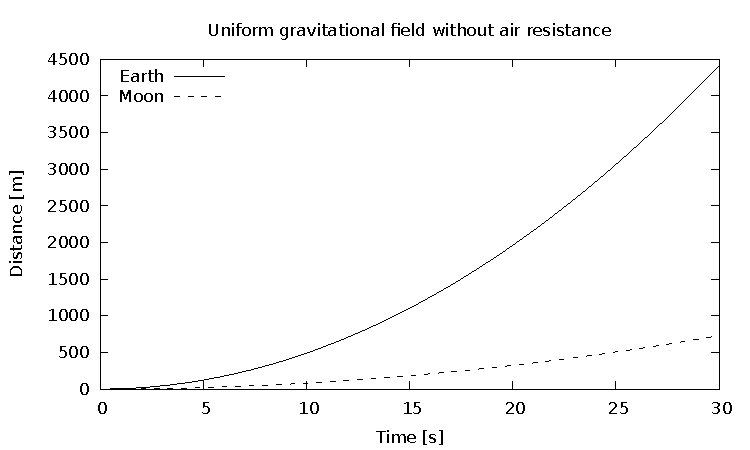
\includegraphics{gnuplot-bw}
% 	\caption{Černobílá varianta obrázku generovaného programem Gnuplot}\label{fig:gnuplot-bw}
% \end{figure}
% 
% \begin{figure}\centering
% 	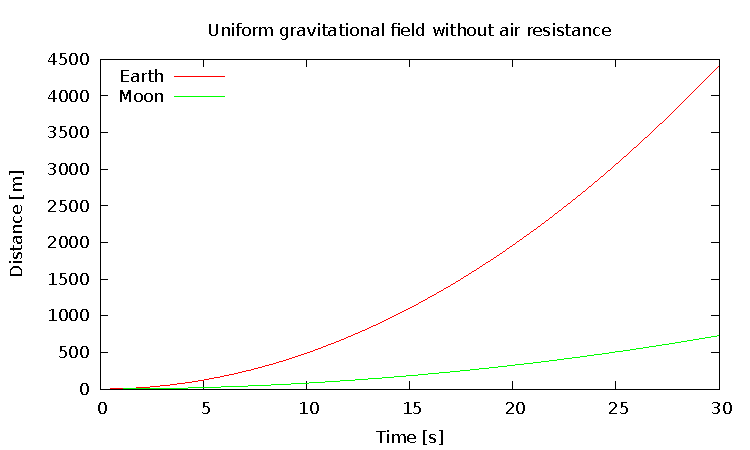
\includegraphics{gnuplot-col}
% 	\caption{Barevná varianta obrázku generovaného programem Gnuplot}\label{fig:gnuplot-col}
% \end{figure}
% 
% 
% \subsection{Tabulky}
% 
% Tabulky lze zadávat různě, např. v~prostředí \verb|tabular|, avšak pro jejich vkládání platí to samé, co pro obrázky -- použijte plovoucí prostředí, v~tomto případě \verb|table|. Například tabulka \ref{tab:matematika} byla vložena tímto způsobem.
% 
% \begin{table}\centering
% 	\caption[Příklad tabulky]{Zadávání matematiky}\label{tab:matematika}
% 	\begin{tabular}{|l|l|c|c|}\hline
% 		Typ		& Prostředí		& \LaTeX{}ovská zkratka	& \TeX{}ovská zkratka	\tabularnewline \hline \hline
% 		Text		& \verb|math|		& \verb|\(...\)|	& \verb|$...$|		\tabularnewline \hline
% 		Displayed	& \verb|displaymath|	& \verb|\[...\]|	& \verb|$$...$$|	\tabularnewline \hline
% 	\end{tabular}
% \end{table}
% 
% % % % % % % % % % % % % % % % % % % % % % % % % % % % 

\chapter{Obsah přiloženého CD}

%upravte podle skutecnosti

\begin{figure}
	\dirtree{%
		.1 readme.txt\DTcomment{stručný popis obsahu CD}.
		.1 exe\DTcomment{adresář se spustitelnou formou implementace}.
		.1 src.
		.2 impl\DTcomment{zdrojové kódy implementace}.
		.2 thesis\DTcomment{zdrojová forma práce ve formátu \LaTeX{}}.
		.1 text\DTcomment{text práce}.
		.2 thesis.pdf\DTcomment{text práce ve formátu PDF}.
		.2 thesis.ps\DTcomment{text práce ve formátu PS}.
	}
\end{figure}

\end{document}
